\item{ 
\textbf{\enfr{ Feature Maps}{ Fonctions de transformation des données}}
\points{8}{8}


\enfr{
In this exercise, you will design feature maps to transform an original dataset into a linearly separable set of points. For the following questions, if your answer is `\textit{yes}', write the expression for the proposed transformation; and if your answer is `\textit{no}', write a brief explanation. You are expected to provide explicit formulas for the feature maps, and these formulas should only use common mathematical operations.
}{
Dans cet exercice, vous allez concevoir des fonctions de transformation depuis l'espace de traits caractéristiques original vers un espace où les données sont linéairement séparables. Pour les questions suivantes, si vous répondez `\textit{oui}', écrivez l'expression de la transformation correspondante; et si votre réponse est `\textit{non}', ajoutez une courte justification de votre réponse. Vous devez donner les formules explicites des transformations, et ces formules doivent utiliser uniquement des opérations mathématiques simples.
}


\begin{enumerate}
    \item { [2 points] \enfr{
    Consider the following 1-D dataset (Figure \ref{a}). Can you propose a 1-D transformation that will make the points linearly separable?
    }{
    Soit les données 1-D suivantes (Figure \ref{a}). Pouvez-vous proposer une transformation 1-D (i.e. vers un espace de dimension 1) qui rend les points linéairement séparables?
    }

    \begin{figure}[!h]
    \centering
    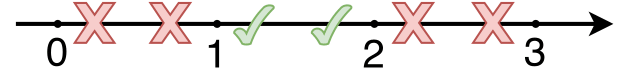
\includegraphics[width=0.55\textwidth]{2/theory/Fig1.png}
    \caption{1D dataset}
    \label{a}
    \end{figure}}
%     \item {[2 points] In the same dataset, can you propose a 2-D transformation that makes the points linearly separable?}

    \item { [2 points] 
    \enfr{
    Consider the following 2-D dataset (Figure \ref{b}). Can you propose a transformation into 1D that will make the data linearly separable? 
    }{
    Soit les données 2-D suivantes (Figure \ref{b}). Pouvez-vous proposer une transformation 1-D qui rend les points linéairement séparables?
    }
    \begin{figure}[h]
    \centerline{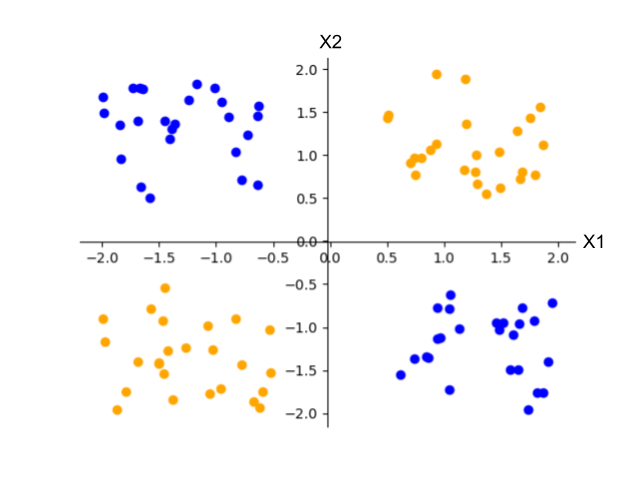
\includegraphics[scale=0.4]{2/theory/Fig2.png}}
    \caption{2D dataset}
    \label{b}
    \end{figure}}

    \item { [4 points] 
    \enfr{
    Using ideas from the above two datasets, can you suggest a transformation of the following dataset (as shown in Figure \ref{12}) that makes it linearly separable? If `\textit{yes}', also provide the kernel corresponding to the feature map you proposed. 
    }{
    En utilisant les idées que vous avez utilisées pour les deux questions précédentes, pouvez-vous proposer une transformation 2-D des données suivantes (Figure \ref{12}) qui les rendent linéairement séparables? Si votre réponse est `\textit{oui}', donnez l'expression du noyau qui correspond à la transformation proposée.
    }
    \begin{figure}[ht]
    \centering
    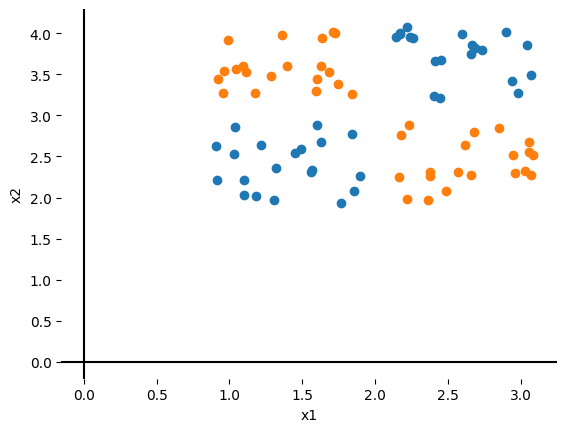
\includegraphics[scale=0.5]{2/theory/Fig3.png}
    \caption{Another 2D dataset}
    \label{12}
    \end{figure}}
    
\end{enumerate} 
}
